% -*- mode: latex; -*-
\DocumentMetadata{pdfstandard=X-4p}
\documentclass[aspectratio=169,8pt]{beamer}
\usetheme{metropolis}

% Standard packages

\usepackage[english]{babel}
%\usepackage[latin1]{inputenc}
%\usepackage{times}
%\usepackage[T1]{fontenc}
\usepackage{fontspec}
\usepackage[]{unicode-math}
\setsansfont{Roboto}
\usepackage{amsmath}

% Setup asymptote
\usepackage[inline]{asymptote}

\newcounter{counter}
% Author, Title, etc.

\title{[E]XOR Linked List}

\author[Shiv Shankar Dayal]{Shiv Shankar Dayal}

\begin{document}
\begin{frame}
  \titlepage
\end{frame}
\begin{frame}{XOR Linked List}
  XOR or EXOR linked lists are memory efficient lists because instead of storing two
  pointers it stores XOR or next and previous nodes' addresses. It is usefull in
  memory constrained environment like embedded devices. In general, it is not worth using
  due to its complicated code compared to normal linked list because memory is quiet
  cheap and plentiful on modern devices.
  \begin{center}
    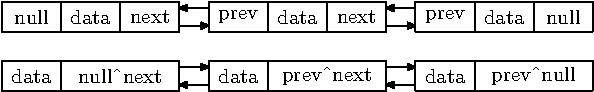
\includegraphics{exor_linked_list}
  \end{center}
  \begin{itemize}
  \item {\bf Singly XOR Linked List:} In this linked list each node stores the XOR of
  current and next node.
  \item{\bf Doubly XOR Linked List:} In this linked list each node stores the XOR of
  next and previours nodes.
  \end{itemize}
\end{frame}
\end{document}
